%=====================================================================
%  MODELO DE RELATÓRIO FINAL DE SUBPROJETO DE INICIAÇÃO CIENTÍFICA
%  Programa Institucional de Iniciação Científica – Piic/UFES
%
%  Versão LaTeX do modelo .docx oficial. Compilar com pdfLaTeX.
%  Formatação exigida pelo modelo:
%    - A4, margens 3 cm (esquerda e superior) e 2 cm (direita e inferior)
%    - Times New Roman 10 pt, espaçamento 1,5, justificado, sem recuo
%    - Títulos de seção: Times 12 pt
%    - Cabeçalho: Times 9 pt, alinhado à direita, 4 linhas
%    - Máximo de 15 páginas
%=====================================================================
\documentclass[10pt,a4paper]{article}

%---------------------------------------------------------------------
% Codificação, idioma e fonte
%---------------------------------------------------------------------
\usepackage[utf8]{inputenc}
\usepackage[T1]{fontenc}
\usepackage[brazil]{babel}
\IfFileExists{newtxtext.sty}{%
  \usepackage{newtxtext}
  \usepackage{newtxmath}
}{%
  \usepackage{mathptmx}
}
\usepackage{amsmath}
\usepackage{microtype}

%---------------------------------------------------------------------
% Página, cabeçalho e rodapé
%---------------------------------------------------------------------
\usepackage[a4paper,left=3cm,top=3cm,right=2cm,bottom=2cm,
            headheight=46pt,headsep=14pt,footskip=28pt]{geometry}
\usepackage{setspace}
\onehalfspacing
\setlength{\parindent}{0pt}
\setlength{\parskip}{0pt}
\usepackage{fancyhdr}
\usepackage{xcolor}
\usepackage{graphicx}
\usepackage{tabularx}
\usepackage{array}
\usepackage{booktabs}
\usepackage{enumitem}
\usepackage{caption}
\usepackage{titlesec}
\usepackage[hidelinks]{hyperref}

%---------------------------------------------------------------------
% DADOS DO RELATÓRIO — preencha aqui
%---------------------------------------------------------------------
% Grande Área do Conhecimento (CNPq): Ciências Exatas e da Terra;
% Ciências Biológicas; Engenharias; Ciências da Saúde; Ciências Agrárias;
% Ciências Sociais Aplicadas; Ciências Humanas; Linguística, Letras e Artes.
\newcommand{\grandeArea}{Grande Área do Conhecimento (CNPq)}
\newcommand{\tituloSubprojeto}{Título do Subprojeto de Iniciação Científica -- Piic/UFES}
\newcommand{\edital}{Edital Piic 20\underline{\hspace{0.6cm}}/20\underline{\hspace{0.6cm}}}
\newcommand{\areaConhecimento}{}
\newcommand{\tituloProjeto}{}
\newcommand{\orientador}{}
\newcommand{\estudante}{}

% No modelo original, o cabeçalho e o título aparecem em vermelho e devem
% ser trocados para preto ao preencher. Troque \placeholderColor por
% "black" quando os campos acima estiverem preenchidos.
\newcommand{\placeholderColor}{red}

%---------------------------------------------------------------------
% Cabeçalho (Times 9 pt, à direita) e rodapé (número da página)
%---------------------------------------------------------------------
\pagestyle{fancy}
\fancyhf{}
\renewcommand{\headrulewidth}{0pt}
\fancyhead[R]{\fontsize{9}{11}\selectfont\begin{tabular}[b]{@{}r@{}}
  Universidade Federal do Espírito Santo\\
  Programa Institucional de Iniciação Científica\\
  Relatório Final de Pesquisa\\
  \textcolor{\placeholderColor}{\grandeArea}
\end{tabular}}
\fancyfoot[R]{\fontsize{10}{12}\selectfont\thepage}

%---------------------------------------------------------------------
% Títulos de seção (Times 12 pt, negrito, com linha inferior)
%---------------------------------------------------------------------
\titleformat{\section}
  {\normalfont\fontsize{12}{14}\selectfont\bfseries}
  {\thesection}{1em}{}[\vspace{-0.6ex}\titlerule]
\titlespacing*{\section}{0pt}{2.2ex plus 1ex minus .2ex}{1.6ex plus .2ex}

% Subtítulos da seção de Referências (marcador ● + negrito)
\titleformat{\subsubsection}
  {\normalfont\fontsize{10}{12}\selectfont\bfseries}
  {}{0pt}{\textbullet\,}
\titlespacing*{\subsubsection}{0pt}{2ex plus .5ex}{0.5ex}

%---------------------------------------------------------------------
% Figuras, gráficos, tabelas e quadros (ABNT: título em cima, fonte embaixo)
%---------------------------------------------------------------------
\DeclareCaptionType{grafico}[Gráfico][Lista de Gráficos]
\DeclareCaptionType{quadro}[Quadro][Lista de Quadros]
\captionsetup{labelsep=endash,justification=raggedright,singlelinecheck=false,
              font=normalsize,position=top,skip=4pt}

% \fonte{...} e \nota{...} : alinhados à borda esquerda do elemento.
% Use dentro de um \begin{minipage}{<largura do elemento>} para que a
% fonte fique limitada pela largura da ilustração/tabela.
\newcommand{\fonte}[1]{\par\vspace{2pt}{\small\singlespacing\raggedright Fonte: #1\par}}
\newcommand{\nota}[1]{{\small\singlespacing\raggedright Nota: #1\par}}

%---------------------------------------------------------------------
% Listas
%---------------------------------------------------------------------
\setlist{nosep,topsep=2pt}
\setlist[itemize]{label=\textbullet,leftmargin=2.2em}
\setlist[enumerate]{label=\alph*),leftmargin=2.2em}

%---------------------------------------------------------------------
% Referências: alinhadas à esquerda, espaço simples, separadas por
% uma linha em branco (estilo "Referência" do modelo original)
%---------------------------------------------------------------------
\newenvironment{referencias}
  {\begin{list}{}{\setlength{\leftmargin}{2.2em}\setlength{\itemsep}{\baselineskip}
     \setlength{\parsep}{0pt}\setlength{\topsep}{4pt}}
   \singlespacing\raggedright\sloppy}
  {\end{list}}
\newcommand{\referencia}{\item[]}
\newcommand{\exemplos}{\item[]{\itshape Exemplos:}\vspace{-\baselineskip}}
\newcommand{\exemplo}{\item[]{\itshape Exemplo:}\vspace{-\baselineskip}}

\newcolumntype{L}{>{\raggedright\arraybackslash}X}

%=====================================================================
\begin{document}

%---------------------------------------------------------------------
% Título e quadro de identificação
%---------------------------------------------------------------------
\begin{center}
  {\fontsize{14}{17}\selectfont\bfseries\textcolor{\placeholderColor}{\tituloSubprojeto}\par}
\end{center}
\vspace{4pt}

\begin{table}[h!]
  \centering\singlespacing
  \begin{tabularx}{\textwidth}{|>{\bfseries}p{0.42\textwidth}|L|}
    \hline
    Edital: & \textbf{\edital} \\ \hline
    Grande Área do Conhecimento (CNPq): & \grandeArea \\ \hline
    Área do Conhecimento (CNPq): & \areaConhecimento \\ \hline
    Título do Projeto: & \tituloProjeto \\ \hline
    Título do Subprojeto: & \tituloSubprojeto \\ \hline
    Professor Orientador: & \orientador \\ \hline
    Estudante: & \estudante \\ \hline
  \end{tabularx}
\end{table}

%---------------------------------------------------------------------
\section*{Resumo}
%---------------------------------------------------------------------
A NBR 6028:2003 estabelece os requisitos para redação e apresentação de resumos, definindo-os como sendo uma ``apresentação concisa dos pontos relevantes de um documento'' (Associação Brasileira de Normas Técnicas, 2003, p.~1). No caso do Relatório Final de Pesquisa, este resumo seria do tipo informativo, isto é, que deve informar ao leitor uma breve contextualização do tema do trabalho realizado, as justificativas, os objetivos, a metodologia adotada, os resultados obtidos, e as conclusões. O texto do resumo deve ser composto de uma sequência de frases concisas, afirmativas (e não de enumeração de tópicos), em um parágrafo único. Por outro lado, devem-se evitar citações, símbolos e contrações que não sejam de uso corrente, bem como fórmulas, equações, diagramas e etc. Quanto à sua extensão, o Resumo deve ter de 150 a 200 palavras.

\vspace{\baselineskip}
\textbf{Palavras-chave:} As palavras-chave devem figurar logo abaixo do resumo, antecedidas da expressão ``Palavras-chave:'', separadas entre si por ponto e finalizadas também por ponto. Devem fornecer ao leitor uma ideia dos principais temas de interesse de que trata a pesquisa. Podem ser informadas, no máximo, 06 (seis) palavras chave.

%---------------------------------------------------------------------
\section{Introdução}
%---------------------------------------------------------------------
Este documento deve ser utilizado como modelo para a elaboração do Relatório Final de Pesquisa no âmbito do Programa Institucional de Iniciação Científica (Piic) da Ufes. Deve ser composto das seguintes seções: resumo, introdução, objetivos, referencial teórico, metodologia, resultados, conclusões e referências bibliográficas.

\vspace{\baselineskip}
O texto do Relatório Final de Pesquisa deve ser preparado considerando que todas as seções que compõem o documento não excedam 15 páginas de formato A4 com margens de 3~cm (esquerda e superior) e de 2~cm (direita e inferior), usando fonte Times New Roman, tamanho da fonte 10, com espaçamento entre linhas de 1,5, sem recuo na primeira linha de cada parágrafo e com alinhamento justificado. Já os títulos das seções também devem utilizar a fonte Times New Roman, mas com tamanho 12. Por fim, o cabeçalho de todas as páginas deve ser mantido de acordo com a formatação deste modelo (Times New Roman, tamanho 9, alinhado à direita), sendo que a quarta linha do cabeçalho deve ser alterada para a cor preto e descrever a Grande Área do Conhecimento do projeto segundo o Conselho Nacional de Desenvolvimento Científico e Tecnológico (CNPq), isto é, Ciências Exatas e da Terra, Ciências Biológicas, Engenharias, Ciências da Saúde, Ciências Agrárias, Ciências Sociais Aplicadas, Ciências Humanas ou Linguística, Letras e Artes. O título do Subprojeto de Iniciação Científica deve ser inserido no lugar de ``Título do Subprojeto de Iniciação Científica -- Piic/UFES'' e sua cor, também trocada para preto.

\vspace{\baselineskip}
Por outro lado, a linguagem utilizada ao longo do trabalho deve ser técnica e impessoal, afinal, trata-se de um trabalho acadêmico. Deve-se evitar o uso de gírias e de termos de linguagem coloquial, bem como o uso de concordâncias nas primeiras pessoas do singular e do plural (fiz ou fizemos\ldots; obtive ou obtivemos\ldots). Nestes casos, deve-se utilizar da impessoalidade por meio do uso da terceira pessoa (fez-se\ldots; foram obtidos\ldots).

\vspace{\baselineskip}
O conteúdo de cada seção deve estar de acordo com as recomendações descritas neste modelo. Na Introdução, o autor deve apresentar uma contextualização do tema de sua pesquisa, mostrando sua relevância, justificando o tema escolhido, e descrevendo claramente a sua pergunta de pesquisa ou problema de pesquisa, citando, sempre que possível, trabalhos de outros autores. Nesta seção, deve-se também ressaltar a ligação do Subprojeto de Iniciação Científica com o Projeto de Pesquisa ao qual está vinculado.

%---------------------------------------------------------------------
\section{Objetivos}
%---------------------------------------------------------------------
A seção Objetivos deve conter, de forma concisa, quais foram os objetivos geral e específicos do Subprojeto de Iniciação Científica, ou seja, as hipóteses que se quis demonstrar, os dispositivos que se quis montar, os compostos que se desejava sintetizar, as ideias que se desejava corroborar ou refutar e etc. Também deve apresentar, de forma concisa, as razões pelas quais se desejava atingir estes objetivos.

%---------------------------------------------------------------------
\section{Embasamento Teórico}
%---------------------------------------------------------------------
De acordo com Prodanov e Freitas (2013, p.~130--133), o ``Embasamento Teórico'' compreende ``elementos de fundamentação teórica da pesquisa e, também, a definição dos conceitos empregados'' à realização do trabalho. Os elementos de fundamentação teórica da pesquisa, a revisão da bibliografia e a definição dos termos e conceitos aplicados na pesquisa devem ser aqui reportados.

\vspace{\baselineskip}
Normalmente, há várias citações nesta seção, que são trechos transcritos ou informações retiradas de outras fontes (escrita ou oral), inseridos no texto com o propósito de esclarecer, complementar e até mesmo sustentar as ideias do autor do trabalho. Como se tratam de informações de autoria diferente do trabalho acadêmico em questão, a fonte de onde foi extraída deve ser obrigatoriamente identificada para fins de garantia e respeito dos direitos autorais. Todas as obras citadas no texto devem fazer parte da lista de referências na seção ``Referências Bibliográficas'', seguindo as regras de apresentação definidas na ABNT NBR 6023:2018.

\vspace{\baselineskip}
As citações podem acontecer de três formas distintas ao longo do trabalho:
\begin{enumerate}
  \item \textbf{Citação direta} -- quando é feita a transcrição literal de textos de outros autores. Ou seja, utilizam-se as mesmas palavras do autor consultado no texto que está sendo escrito;
  \item \textbf{Citação indireta} -- quando ocorre apenas a reprodução da ideia sem a transcrição literal do texto do autor consultado. Neste caso, as palavras utilizadas no texto que está sendo escrito são diferentes das adotadas pelo autor consultado, mas a ideia (informação) transmitida é a mesma;
  \item \textbf{Citação de citação} -- nos casos em que não for possível consultar o documento original, pode-se fazer a transcrição (direta ou indireta) de uma informação já citada por outros autores. No entanto, todo esforço deve ser empreendido para que a fonte original da informação seja consultada antes de se utilizar desse tipo de citação.
\end{enumerate}

\vspace{\baselineskip}
Neste Relatório Final de Pesquisa, a identificação das citações deve ser incluída no texto e a chamada das mesmas deve utilizar o sistema autor-data, tudo conforme a ABNT NBR 10520:2002 (Associação Brasileira de Normas Técnicas, 2002).

%---------------------------------------------------------------------
\section{Metodologia}
%---------------------------------------------------------------------
A metodologia que foi adotada para testar a hipótese formulada e atingir os objetivos estabelecidos deve ser aqui detalhada, classificando a pesquisa realizada do ponto de vista da sua natureza, dos seus objetivos, dos procedimentos técnicos e da forma de abordagem do problema de pesquisa. Necessita ainda apresentar os procedimentos de trabalho, os materiais que foram utilizados, o tratamento da informação realizado e o procedimento estatístico aplicado, se for o caso. Esta seção deve, entretanto, além de detalhar os aspectos da metodologia empregada nas atividades especificamente executadas pelo estudante, apresentar sua relação com o Projeto de Pesquisa ao qual o Subprojeto de Iniciação Científica está vinculado.

%---------------------------------------------------------------------
\section{Resultados e Discussão}
%---------------------------------------------------------------------
Esta seção deve explicitar os resultados ou respostas encontradas durante o trabalho de pesquisa, apresentando os dados/informações obtidos(as) ou coletados(as) e incluindo ilustrações, figuras, fotos ou esquemas.

\vspace{\baselineskip}
Além de expor os resultados encontrados, os mesmos devem ser interpretados, analisados e relacionados com o ``Embasamento Teórico'' existente e abordado anteriormente na seção~3. Ou seja, deve haver uma discussão sobre o significado dos resultados obtidos, contemplando, preferencialmente, os seguintes aspectos:
\begin{itemize}
  \item O que estas respostas ou dados obtidos significam?
  \item Como elas ajudam a resolver o problema?
  \item Descrição dos dados à luz da literatura, isto é, como as respostas obtidas se comparam com os dados de literatura.
  \item Quais as possíveis fontes de erro e seu efeito sobre os dados ou análises?
\end{itemize}

\vspace{\baselineskip}
Quanto às ilustrações (figuras, gráficos, fluxogramas, quadros e etc.) e tabelas, estas devem ser utilizadas a fim de explicar ou complementar visualmente o texto. Desta forma, torna-se obrigatória a inclusão de um comentário sobre a ilustração ou a tabela no texto. A NBR 15287:2011 reforça este fato quando diz que ``A ilustração deve ser citada no texto e inserida o mais próximo possível do trecho a que se refere.'' (Associação Brasileira de Normas Técnicas, 2011, p.~8). Cabe ressaltar que a citação no texto sempre deve preceder a ilustração ou a tabela. Estes elementos devem estar centralizados na página, sua identificação na parte superior e a indicação da fonte consultada (elemento obrigatório, mesmo que seja produção do próprio autor), legenda, notas e outras informações necessárias à sua compreensão (se houver), na parte inferior (alinhados à borda esquerda da ilustração e limitados pela borda direita da mesma), como mostram a Figura~\ref{fig:edificacao} e o Gráfico~\ref{graf:energia}.

\begin{figure}[htbp]
  \centering
  \begin{minipage}{0.75\textwidth}
    \caption{(a) Fotografia do modelo de edificação utilizado no experimento e (b) representação esquemática do comportamento do escoamento sobre a edificação}
    \label{fig:edificacao}
    \centering
    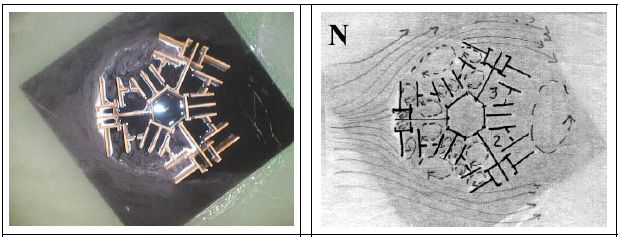
\includegraphics[width=\linewidth]{figura1.png}\\[-2pt]
    {\small \makebox[0.4\linewidth]{(a)}\hfill\makebox[0.4\linewidth]{(b)}}
    \fonte{Toledo e Pereira (2004).}
  \end{minipage}
\end{figure}

\begin{grafico}[htbp]
  \centering
  \begin{minipage}{0.7\textwidth}
    \caption{Consumo final de energia por fonte no Brasil em 2011}
    \label{graf:energia}
    \centering
    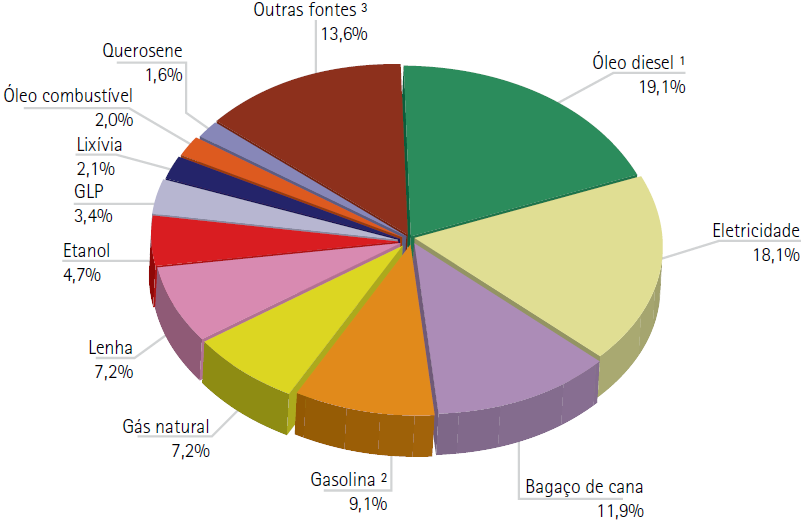
\includegraphics[width=\linewidth]{grafico1.png}
    \fonte{Empresa de Pesquisa Energética (2012).}
    \nota{\textsuperscript{1}~Inclui biodiesel. \textsuperscript{2}~Inclui apenas gasolina A (automotiva). \textsuperscript{3}~Inclui gás de refinaria, coque de carvão mineral e carvão vegetal, dentre outros.}
  \end{minipage}
\end{grafico}

As tabelas e os quadros, apesar de possuírem certa semelhança entre si, diferenciam-se não apenas no formato exigido, mas também pelo conteúdo que exibem:
\begin{enumerate}
  \item um quadro apresenta informações ou resultados qualitativos, ou seja, em forma de texto, mesmo que este empregue números;
  \item uma tabela apresenta informações ou resultados quantitativos, ou seja, números tratados estatisticamente.
\end{enumerate}

\vspace{\baselineskip}
Quanto ao formato e à apresentação de tabelas e quadros, como se verifica na Tabela~\ref{tab:exemplo} e no Quadro~\ref{qua:boost}, devem-se observar as seguintes regras (Fundação Instituto Brasileiro de Geografia e Estatística, 1993):
\begin{enumerate}
  \item a moldura das tabelas não deve ser fechada com traços verticais à esquerda e à direita;
  \item deve-se evitar o uso de traços verticais para separar as colunas e de traços horizontais para separar as linhas de uma tabela;
  \item o quadro é um elemento fechado, portanto, deve conter traços horizontais e verticais para separar suas linhas e colunas, além de traços horizontais e verticais para delimitar sua moldura.
\end{enumerate}

\begin{table}[htbp]
  \centering\singlespacing
  \begin{minipage}{0.86\textwidth}
    \caption{Exemplo de formatação de uma tabela para a apresentação de resultados}
    \label{tab:exemplo}
    \centering
    \begin{tabular}{ccc}
      \toprule
      \textbf{Grupos de idade [meses]} & \textbf{Número de indivíduos no grupo} & \textbf{Indivíduos viáveis [\%]} \\
      \midrule
      0 -- 10     & 20 & 9,0 \\
      10 -- 15    & 20 & 10,0 \\
      15 -- 20    & 25 & 4,0 \\
      Acima de 20 & 15 & 3,4 \\
      \bottomrule
    \end{tabular}
    \fonte{Produção do(a) próprio(a) autor(a).}
  \end{minipage}
\end{table}

\begin{quadro}[htbp]
  \centering\singlespacing
  \begin{minipage}{0.6\textwidth}
    \caption{Dimensionamento dos elementos de um conversor \textit{boost}}
    \label{qua:boost}
    \centering
    \begin{tabular}{|l|l|}
      \hline
      \textbf{Elemento ou Grandeza} & \textbf{Valor ou Modelo} \\ \hline
      Tensão de entrada        & 48 V \\ \hline
      Tensão de saída          & 200 V \\ \hline
      Potência de saída        & 200 W \\ \hline
      Frequência de comutação  & 50 kHz \\ \hline
      Indutor de entrada       & 880 $\mu$H \\ \hline
      Capacitor de saída       & 22 $\mu$F \\ \hline
      Diodo                    & FES8HT \\ \hline
      Interruptor              & IRFP360 \\ \hline
    \end{tabular}
    \fonte{Menegáz (1997).}
  \end{minipage}
\end{quadro}

Outros elementos textuais que podem fazer parte do Relatório de Pesquisa são as equações e fórmulas. Para facilitar a leitura, a NBR 15287:2011 exige que as equações sejam destacadas do texto e numeradas com algarismos arábicos entre parênteses, alinhados à margem direita da página, como mostra a equação~\eqref{eq:ohm}. Assim como no caso de figuras, tabelas e quadros, a citação, ou a chamada, de todas as equações ou fórmulas no texto é obrigatória, e sua localização deve acontecer o mais próximo possível do trecho onde são mencionadas pela primeira vez.
\begin{equation}
  v_r(t) = R \times i(t)
  \label{eq:ohm}
\end{equation}

%---------------------------------------------------------------------
\section{Conclusões}
%---------------------------------------------------------------------
Esta seção é a parte final do Relatório de Pesquisa onde são apresentadas conclusões correspondentes aos objetivos e/ou às hipóteses do trabalho, explicitando a resposta à pergunta do problema de investigação e as possíveis limitações da pesquisa realizada. Deve ainda conter:
\begin{itemize}
  \item Uma compilação dos resultados dos resultados da pesquisa feita;
  \item Quais as principais dificuldades e limitações encontradas durante o estudo;
  \item As contribuições que o estudo proporcionou nos âmbitos acadêmico, profissional e da sociedade;
  \item Se seus experimentos ou análises falharam, quais as sugestões para corrigir o problema;
  \item Quais as perspectivas ou sugestões de continuidade do trabalho.
\end{itemize}

\vspace{\baselineskip}
Opcionalmente, conforme as especificidades de cada Grande Área do Conhecimento, o autor pode utilizar a seção~5 para apenas apresentação de resultados, deixando a seção~6 para a discussão dos resultados e as conclusões. Neste caso, o título da seção~5 deverá ser ``Resultados'' e da seção~6, ``Discussão e Conclusões''.

\vspace{\baselineskip}
Por fim, cabe ainda ressaltar que o Relatório Final é individual e deve ser escrito pelo discente bolsista/voluntário de iniciação científica, sob a supervisão/orientação do seu professor orientador. O relatório deverá ser enviado pelo orientador utilizando o Sistema Acadêmico de Pesquisa e Pós-Graduação (SAPPG), a partir do dia de início de envio até a data limite estabelecidos no Edital. O envio do Relatório Final após a data limite fixada implicará nas sanções previstas ao orientador e seu orientando, conforme estabelecido em Edital e no Regulamento Geral do Piic/UFES, disponível no site da Pró-Reitoria de Pesquisa e Pós-Graduação (PRPPG).

%---------------------------------------------------------------------
\section*{Agradecimentos}
%---------------------------------------------------------------------
Esta é uma seção opcional e deve ser utilizada para registrar os agradecimentos do autor do Subprojeto de Iniciação Científica pelo suporte técnico e/ou financeiro recebido de instituições públicas ou privadas. Caso não haja agradecimentos a serem feitos, esta seção deve ser excluída do Relatório Final.

%---------------------------------------------------------------------
\section*{Referências Bibliográficas}
%---------------------------------------------------------------------
Esta seção deve descrever as fontes consultadas durante a realização do Subprojeto de Iniciação Científica, seguindo a norma técnica pertinente, a saber a NBR 6028:2003. Deve conter apenas as obras citadas no texto, ou seja, ``não liste se não citar'' e ``não cite se não listar''. Por outro lado, a lista das referências bibliográficas deve estar em ordem alfabética.

\vspace{\baselineskip}
``As referências são alinhadas somente à margem esquerda do texto e de forma a se identificar individualmente cada documento, em espaço simples e separadas entre si por uma linha em branco de espaço simples.'' (Associação Brasileira de Normas Técnicas, 2018, p.~5), ou seja, por uma linha em branco. Esta formatação está definida nesse modelo como o ambiente \texttt{referencias}.

\vspace{\baselineskip}
A seguir, são apresentados os elementos essenciais das referências de alguns tipos de documentos, seguidos de alguns exemplos. No caso de outros tipos de publicação, deve-se consultar a NBR 6023:2018.

\subsubsection*{Monografias no todo}
Nessa classe estão incluídos os livros, manuais, guias, catálogos e trabalhos acadêmicos (trabalhos de conclusão de curso, dissertações e teses), entre outros. Segundo a NBR 6023:2018, o padrão a ser seguido nesses casos é:
\begin{enumerate}
  \item livros:
\end{enumerate}
\begin{referencias}
  \referencia SOBRENOME DO AUTOR, Prenome. \textbf{Título}: subtítulo (se houver). Edição (se houver). Local: Editora, ano de publicação.
  \exemplos
  \referencia PRODANOV, C. C.; FREITAS, E. C. \textbf{Metodologia do trabalho científico}: Métodos e Técnicas da Pesquisa e do Trabalho Acadêmico. 2. ed. Novo Hamburgo: Feevale, 2013.
  \referencia FUNDAÇÃO INSTITUTO BRASILEIRO DE GEOGRAFIA E ESTATÍSTICA. Centro de Documentação e Disseminação de Informações. \textbf{Normas de apresentação tabular}. 3. ed. Rio de Janeiro: IBGE, 1993.
  \referencia EMPRESA DE PESQUISA ENERGÉTICA. \textbf{Balanço Energético Nacional -- Ano Base 2011}: Resultados preliminares. Rio de Janeiro: EPE, 2012.
\end{referencias}
\begin{enumerate}[resume]
  \item trabalhos acadêmicos:
\end{enumerate}
\begin{referencias}
  \referencia SOBRENOME DO AUTOR, Prenome. \textbf{Título}: subtítulo (se houver). Ano de depósito. Tipo de trabalho \textit{(tese, dissertação, monografia, trabalho de conclusão de curso e outros)} (Grau \textit{(doutorado, mestrado, especialização, graduação, bacharelado, licenciatura, entre outros)} e Curso) -- Vinculação acadêmica, local e ano de apresentação ou defesa \textit{(mencionado na folha de aprovação)}.
  \exemplos
  \referencia FERNANDES, R. O. \textbf{Aplicação do método de Morgan para cálculo de capacidade de linhas de transmissão em Alta Tensão}. 2009. Trabalho de Conclusão de Curso (Graduação em Engenharia Elétrica) -- Centro Tecnológico, Universidade Federal do Espírito Santo, Vitória, 2009.
  \referencia MENEGÁZ, P. J. M. \textbf{Uso de acoplamento magnético na melhoria de características de algumas estruturas ZVT}. 2005. Tese (Doutorado em Engenharia Elétrica) -- Programa de Pós-Graduação em Engenharia Elétrica, Centro Tecnológico, Universidade Federal do Espírito Santo, Vitória, 2005.
\end{referencias}

\subsubsection*{Parte de monografia}
Seguem a mesma regra apresentada na alínea anterior, acrescentando-se a expressão ``\textit{In}: SOBRENOME, Prenome do responsável pela obra'' e a localização da parte da obra referenciada: capítulo e respectivo número (se houver), página inicial e página final.
\begin{referencias}
  \exemplos
  \referencia ROMANO, Giovanni. Imagens da juventude na era moderna. \textit{In:} LEVI, G.; SCHMIDT, J. (org.). \textbf{História dos jovens 2}: a época contemporânea. São Paulo: Companhia das Letras, 1996. p. 7-16.
  \referencia SANTOS, F. R. A colonização da terra do Tucujús. \textit{In:} SANTOS, F. R. \textbf{História do Amapá, 1º grau}. 2. ed. Macapá: Valcan, 1994. p. 15-24.
  \referencia RODRIGUES, Ana Lúcia Aquilas. Aspectos éticos. \textit{In:} RODRIGUES, Ana Lúcia Aquilas. \textbf{Impacto de um programa de exercícios no local de trabalho sobre o nível de atividade física e o estágio de prontidão para a mudança de comportamento}. 2009. Dissertação (Mestrado em Fisiopatologia Experimental) -- Faculdade de Medicina, Universidade de São Paulo, São Paulo, 2009. f. 19-20.
\end{referencias}

\subsubsection*{Publicação periódica}
Estão incluídos nessa classe revistas, jornais e boletins. Nesses casos, é mais comum fazer referência a um determinado artigo da revista ou do jornal do que referenciar a obra como todo. Assim sendo, de acordo com a Associação Brasileira de Normas Técnicas (2018), o padrão a ser seguido é:
\begin{enumerate}
  \item artigos em revistas técnicas:
\end{enumerate}
\begin{referencias}
  \referencia SOBRENOME DO AUTOR do artigo, Prenome. Título: subtítulo (se houver) do artigo. \textbf{Título do Periódico}, local de publicação, número do ano e/ou volume, número e/ou edição, tomo (se houver), páginas inicial e final do artigo, data (ano) e ou período de publicação.
  \exemplos
  \referencia YONGSOON P.; SEUNG-KI S. A novel method utilizing trapezoidal voltage to compensate for inverter nonlinearity. \textbf{IEEE Transactions on Power Electronics}, [\textit{s. l.}], v. 27, n. 12, p. 4837-4846, dez. 2012.
  \referencia BONINI NETO, A.; ALVES, D. A. Técnicas de parametrização global para o fluxo de carga continuado. \textbf{Controle \& Automação}, Campinas, v. 21, n. 4, p. 323-337, jul./ago. 2010.
\end{referencias}
\begin{enumerate}[resume]
  \item artigos em jornais impressos (inclui comunicação, editorial, entrevista, reportagem, resenha e outros):
\end{enumerate}
\begin{referencias}
  \referencia SOBRENOME DO AUTOR do artigo, Prenome. Título: subtítulo (se houver) do artigo. \textbf{Título do Jornal}: subtítulo do jornal (se houver), local de publicação, numeração do ano e/ou volume, número (se houver), data de publicação. Seção, caderno ou parte do jornal, a paginação correspondente. (Quando não houver seção, caderno ou parte, a paginação do artigo ou matéria precede a data.)
  \exemplo
  \referencia OTTA, Lu Aiko. Parcela do tesouro nos empréstimos do BNDES cresce 566\,\% em oito anos. \textbf{O Estado de S. Paulo}, São Paulo, ano 131, n. 42656, 1 ago. 2010. Economia \& Negócios, p. B1.
\end{referencias}

\subsubsection*{Parte de evento em monografia -- Trabalho apresentado em evento (congressos, seminários, etc.)}
Seguindo o padrão apresentado pela Associação Brasileira de Normas Técnicas (2018), tem-se:
\begin{referencias}
  \referencia SOBRENOME DO AUTOR do artigo, Prenome. Título: subtítulo (se houver) do artigo. \textit{In}: NOME DO EVENTO, numeração do evento (se houver), ano e local (cidade) de realização do evento. \textbf{Título do documento (Anais, Proceedings, Resumos, Atas, \ldots)}. Local: Editora, data (ano) de publicação. Páginas inicial e final da parte referenciada.
  \exemplos
\end{referencias}
\begin{enumerate}
  \item trabalhos impressos:
\end{enumerate}
\begin{referencias}
  \referencia MUMMADI, V. C. Analysis of PV Buck converter supplied DC motors. \textit{In}: CONGRESSO BRASILEIRO DE ELETRÔNICA DE POTÊNCIA, 5., 1999, Foz do Iguaçu. \textbf{Anais} [\ldots]. Foz do Iguaçu: Imprensa Universitária da UFPR, 1999. v. 1, p. 356-360.
\end{referencias}
\begin{enumerate}[resume]
  \item trabalhos em meios eletrônicos:
\end{enumerate}
\begin{referencias}
  \referencia ANDRADE JÚNIOR, M. N.; COSSI, A. M. Planejamento Integrado de Redes de Distribuição de Energia Elétrica. \textit{In}: SIMPÓSIO BRASILEIRO DE SISTEMAS ELÉTRICOS, 4., 2012, Goiânia. \textbf{Anais} [\ldots]. Goiânia: 2012. 1 CD-ROM.
\end{referencias}

\subsubsection*{Normas Técnicas}
De acordo com o padrão apresentado pela Associação Brasileira de Normas Técnicas (2018), tem-se:
\begin{referencias}
  \exemplos
  \referencia ASSOCIAÇÃO BRASILEIRA DE NORMAS TÉCNICAS. \textbf{NBR 6023}: Informação e documentação -- referências -- elaboração. Rio de Janeiro: ABNT, 2018.
  \referencia \rule{1.5cm}{0.4pt}. \textbf{NBR 6028}: Informação e documentação -- resumo -- apresentação. Rio de Janeiro: ABNT, 2003.
  \referencia \rule{1.5cm}{0.4pt}. \textbf{NBR 10520}: Informação e documentação -- citações em documentos -- apresentação. Rio de Janeiro: ABNT, 2002.
  \referencia \rule{1.5cm}{0.4pt}. \textbf{NBR 15287}: Informação e documentação -- projeto de pesquisa -- apresentação. Rio de Janeiro: ABNT, 2011.
\end{referencias}

\subsubsection*{Documentos e publicações \textit{online}}
Além dos elementos essenciais apresentados anteriormente para cada caso, é indispensável a apresentação do endereço eletrônico do documento acessado seguido da data de acesso:
\begin{enumerate}
  \item O endereço eletrônico deve aparecer precedido da expressão ``Disponível em:'';
  \item A data de acesso ao documento deve ser precedida da expressão ``Acesso em:'' (Associação Brasileira de Normas Técnicas, 2018).
\end{enumerate}
\begin{referencias}
  \exemplos
\end{referencias}
\begin{enumerate}
  \item livros:
\end{enumerate}
\begin{referencias}
  \referencia CONSOLI, R. A. G. B.; OLIVEIRA, R. L. \textbf{Principais mosquitos de importância sanitária no Brasil}. Rio de Janeiro: Editora Fiocruz, 1994. 228 p. Disponível em: \url{https://static.scielo.org/scielobooks/th/pdf/consoli-9788575412909.pdf}. Acesso em: 24 maio 2020.
\end{referencias}
\begin{enumerate}[resume]
  \item trabalhos acadêmicos:
\end{enumerate}
\begin{referencias}
  \referencia FILHO, A. S. \textbf{Análise regulatória das condições de interconexão da geração distribuída}: requisitos para os procedimentos de distribuição. 2005. Dissertação (Mestrado em Ciências em Engenharia da Energia) -- Programa de Pós-Graduação em Engenharia da Energia, Universidade Federal de Itajubá, Itajubá, 2005. Disponível em: \url{https://saturno.unifei.edu.br/bim/0029398.pdf}. Acesso em: 29 abr. 2020.
\end{referencias}
\begin{enumerate}[resume]
  \item outros documentos e páginas:
\end{enumerate}
\begin{referencias}
  \referencia ORGANIZAÇÃO DAS NAÇÕES UNIDAS PARA A EDUCAÇÃO, A CIÊNCIA E A CULTURA. \textbf{2012 -- Ano internacional da energia sustentável para todos}. 2012. Disponível em: \url{http://peaunesco-sp.com.br/ano_inter/ano_energia/ano_internacional_da_energia_sustentavel_para_todos_rio_mais_20.pdf}. Acesso em: 25 jun. 2012.
  \referencia EMPRESA DE PESQUISA ENERGÉTICA. \textbf{Balanço Energético Nacional 2018}: Ano base 2017. Rio de Janeiro: EPE, 2018. Disponível em: \url{http://epe.gov.br/sites-pt/publicacoes-dados-abertos/publicacoes/PublicacoesArquivos/publicacao-303/topico-419/BEN2018__Int.pdf}. Acesso em: 29 abr. 2020.
  \referencia YAHOO. \textbf{Gráficos de Mercado}. 2021. Disponível em: \url{http://finance.yahoo.com/chart/GOOG}. Acesso em: 11 maio 2021.
\end{referencias}

\end{document}
